\documentclass[12pt,a4paper]{article}
\usepackage{natbib}
\usepackage{url}
\usepackage{graphicx}
\usepackage{float}
\graphicspath{Images/}
\usepackage{natbib}
\bibliographystyle{agsm}

\title{Artificial Intelligence Assignment: Developing an Intelligent Conversational Bot}
\author{George Markham, Wan-Ju Chen, \\ Anurag Bonde, Owen Birch \\ (Group 4)} %Add your names in here
\date{November 2018}

\begin{document}

    \maketitle
    \section{Introduction}
    The purpose of the chatbot developed for this project is to enable user's to find and book train tickets, find out how long their train is likely to be delayed for, and for train staff to easily access contingency plans in the event of a problem.
    \section{Related Work}
    \section{Design}
    The chatbot will use Facebook's messenger platform as it's interface. Therefore the system will need to be designed around Facebook's requirements. For example it should be designed to run on a server and respond to HTTP requests sent by Facebook. These requests will contain a user's message to the chatbot and the response, therefore, should reflect the user's message. For example if a user sends a message such as "Hi" then the chatbot should respond with a greeting and some information about the chatbot. These responses will be generated on the server side and then sent out to the user. The flowchart below (figure \ref{fig:server_flowchat}) shows how the server will operate.
    
    \begin{figure}[H]
        \centering
        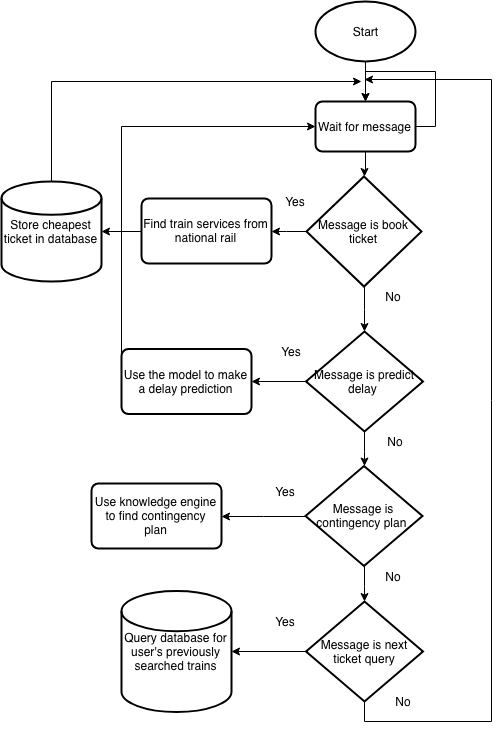
\includegraphics[scale=0.7]{Images/server_flowchart.png}
        \caption{A Flowchart Showing how the Server Should Operate}
        \label{fig:server_flowchat}
    \end{figure}
    
    The flowchart below (\ref{fig:overall_flowchart}) shows how the overall system will work. This is the main guide that was used when developing the chatbot.
    
    \begin{figure}[H]
        \centering
        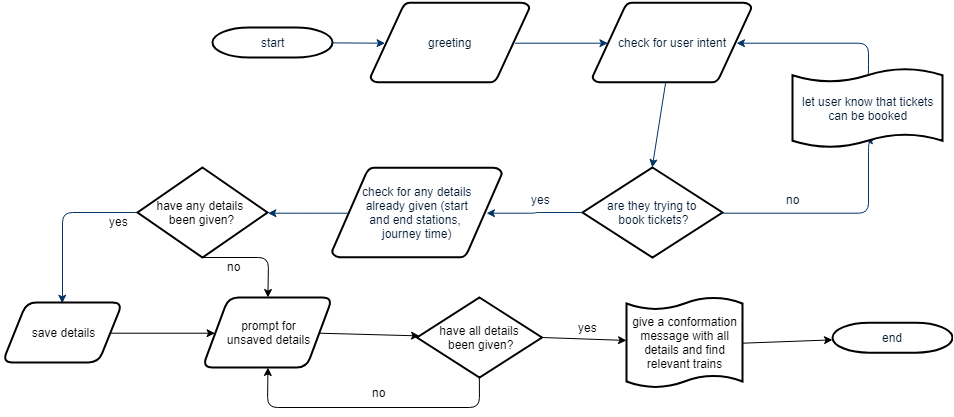
\includegraphics[scale=0.4]{Images/flowchart_overall.png}
        \caption{A Flowchart Showing how the Overall System Should Operate}
        \label{fig:overall_flowchart}
    \end{figure}
    
    \section{Implementation}
    
    To create the chatbot a number of tools and frameworks would need to be used. These would need to be Python based. Currently many of the state of the art machine learning tools such as Keras, TensorFlow, Theano, PyTorch and SciKit Learn are primarily Python based. Therefore, to enable the use of those tools and to allow for the ability to swap and change these tools, one must also use Python. Python also has a lot of support available and a large number of frameworks allowing it to be used for everything this project requires such as server logic.
    
    \subsection{Tools}
    \subsubsection{Facebook Messenger}
    It was decided that, to bring the chatbot to the largest amount of users, Facebook's Messenger platform should be used as our interface. Using Facebook's Messenger platform would allow users to access the chatbot without having to install or sign up to a new service, this was important to the project as the goal is not to give users a new platform rather to provide a service. Facebook also gives a unique ID for each user which can be used for identification in the database.
    
    \subsection{Frameworks}
    
    \subsubsection{DialogFlow}
    DialogFlow provides the natural language processing (NLP) and natural language generation (NLG) for the chatbot. It integrates with Python through a library and therefore gives easy access and allows integration with the rest of the project.
    
    \subsubsection{PyKnow}
    PyKnow is used as the knowledge engine when dealing with contingency plans for train staff. 
    
    \subsubsection{SciKit Learn}
    The SciKit Learn machine learning library provides a number of functions for creating models. SciKit Learn was used to produce the model to predict the delays for a train.
    
    \subsubsection{Flask}
    The Flask Python framework was used to build the server logic that handles the recieving and sending of messages. Flask is easy to use and, as it is Python based, integrates well with the rest of the project.
    
    \subsubsection{BeautifulSoup}
    \label{subsubsection:BeautifulSoup}
    BeautifulSoup is a Python HTML parsing library. This will be used for parsing the National Rail website to get information about trains for the user.
    
    \subsubsection{MongoDB \& PyMongo}
    \label{subsubsection:mongodb}
    It was determined that a document based database would be suitable for this project as there appear to be very few relations and the data collected would not benefit from being stored in seperate tables. MongoDB stores data as binary JSON (BSON) \citep{korneliusz_2014} and as such is relatively quick to read and write. These benefits are good to have and contribute to the use of MongoDB and PyMongo over SQL based relational databases.
    
    \subsection{Server}
    \label{subsection:Server}
    Facebook Messenger requires an SSL encrypted connection to send messages to and receive messages from users. This means that a webserver must be set up with an SSL certifacte in order to facilitate this.
    \subsubsection{Microsoft Azure}
    It was decided to use Microsoft's Azure platform as the host for this project. Azure provides Linux VMs and this allows for proper web server configuration and testing.
    
    \subsubsection{NGINX}
    NGINX was used as a reverse proxy to host the Python application. NGINX passes a connection to the Python Flask application and enables easy SSL certificate generation with Let's Encrypt and the Electronic Frontier Foundation's (EFF) Certbot tool %Link to Let's Encrypt and EFF
    
    \subsubsection{Let's Encrypt}
    Let's Encrypt and EFF's Certbot tool was used to generate the SSL certificate for the server. Certbot automatically configures NGINX to use SSL rather than a standard HTTP connection, making the server configuration much easier.
    
    \subsection{Building the System}
    When developing the system a component based approach was used. Each part of the system was developed independently of the overall system and then put together with the server acting as the entry point and the NLP program acts as the overall controller for the rest of the system. Using this method it can be ensured that each component is fully operational before integrating it into the overall system.
    
    \subsection{Server Logic}
    The server recieves a series of HTTP requests from Facebook when a message is sent. The first is a GET request intended to verify that a) Facebook is the platform sending the message and b) Facebook can verify that the server is the one it is expecting. The Second is a POST request containing the user's information (e.g their unique Sender ID) and their message. The message can then be extracted from this POST request and passed to the NLP component. A POST request is then sent on to Facebook containing the NLG response. This response is passed on to the user as a message.
    
    \subsection{Web Scraping}
    There is no publicly available API to get information about sceduled train journeys in the UK. To get around this a web scraping approach had to be used. A number of websites provide train information (e.g. National Rail and Trailine). It was decided to use the National Rail website to gather train information. The first task was to construct the URL that points to a dynamically generated web page containing the train information. This URL is of the format
    \emph{http://ojp.nationalrail.co.uk/service/timesandfares/FROM/TO/DATE/TIME/dep} where \emph{TO} and \emph{FROM} are the 3 letter station codes (e.g NRW for Norwich), \emph{DATE} is the date formatted as \emph{YYMMDD} (year, month and day concatenated) and \emph{TIME} is the intended travel time formatted as \emph{hhmm} (hour and minute concatenated).
    As stated in \ref{subsubsection:BeautifulSoup} the BeautifulSoup library was used to parse the National Rail website and extract the necessary information such as the train time, date and fare. The trains found on the National Rail website are sorted so that the cheapest one is found first and displayed to the user. Functionality was also built to sort the trains in order of their time of departure however the current version has not made such functionality available to the user.
    
    \subsection{Database}
    
    
    \section{Testing}
    \section{Evaluation}
    \section{Discussion}
    
    \bibliography{main.bib}
    
\end{document}